\documentclass{beamer}

\mode<presentation> {
\usetheme{Madrid}
\usecolortheme{whale}

%\setbeamertemplate{footline} % To remove the footer line in all slides uncomment this line
%\setbeamertemplate{footline}[page number] % To replace the footer line in all slides with a simple slide count uncomment this line
%\setbeamertemplate{navigation symbols}{} % To remove the navigation symbols from the bottom of all slides uncomment this line

}

\usepackage{pdflscape}
\usepackage{booktabs}
\usepackage{geometry}
\usepackage{placeins}
\usepackage{caption}
\usepackage{hyperref}
\usepackage{graphicx}
\usepackage{threeparttable, adjustbox, tabularx, longtable}

\newcommand{\specialcell}[2][c]{\begin{tabular}[#1]{@{}c@{}}#2\end{tabular}}

\title[Lottery]{Using Lotteries to Encourage Saving: Experimental Evidence from Kenya}

\author[Abraham, Akbas, Ariely, Jang (2016)]{Justin Abraham \inst{\ddag} \and Merve Akbas \inst{\dag} \and Dan Ariely \inst{\dag} \and Chaning Jang \inst{\ddag}} \institute[]{\inst{\dag} Duke University \and \inst{\ddag} Princeton University}

\date{\today}

\begin{document}

\begin{frame}
\titlepage
\end{frame}

% joint work with CJ, DA, MA
% name of this project is ``Using Lotteries to Encourage Saving: Experimental Evidence from Kenya''
% one of Busara's earliest projects

\begin{frame} \frametitle{Behavioral Barriers To Saving} \pause

	\begin{itemize}
	\item Why don't people save more? \pause
		\begin{itemize}
		\item Susceptible to extraction (Dupas and Robinson, 2013) \pause
		\item Planning fallacies, self-control, inability to remember \pause
		\end{itemize}
	\item Behaviorally-informed product designs have been extremely cost-effective
		\begin{itemize}
		\item Thaler, 2004; Ashraf, 2006; Karlan, 2010; Kast et al. 2012; Akbas et al. 2016 \pause
		\end{itemize}
	\end{itemize}

\end{frame}

% begin by re-posing a classic development question:
% given high returns to productive investments, the ability to smooth potentially disastrous financial shocks, why don't the poor save more?
% in the absence of proper savings technologies, savings are susceptible to extraction (lack of savings products is a constraint)
% this project focuses on a second explanation: behavioral barriers to savings
% here I'm thinking about planning fallacies, self-control failures, inability to remember
% Behaviorally-informed product designs that target these failures have been extremely cost-effective
% default contributions, binding and non-binding commitment devices, reminders
% previous work by merve and dan showing that using tokens to track can increase savings more than double
% compare these to matched incentives (which incentivize savings in a direct way and are proven to be extremely effective) these little changes in product design are very cheap

\begin{frame} \frametitle{The Promise of LLDAs} \pause
	
	\begin{itemize}
	\item Lottery-linked deposit accounts (LLDAs) incorporate stochastic payoffs to saving \pause
		\begin{itemize}
		\item Has existed since the 17th century and widespread \pause
		\item NS\&I Premium Bonds in the U.K. and A-Million-A-Month in South Africa \pause
		\end{itemize}
	\item How might lotteries better induce savings than a match? \pause
		\begin{itemize}
		\item Over-weighting of small probabilities \pause
		\item Preferences for skewness \pause
		\item Preferences for large payoffs \pause
		\item Hot hand and gambler's fallacy \pause
		\item Thrill of playing \pause
		\end{itemize}
	\end{itemize}

\end{frame}

% want to focus on an specific kind of savings product known as PLSA or LLDA
% kind of savings scheme has been documented in 17th century england
% that incorporates lottery-like incentives to traditional deposit accounts, the opportunity to win large prizes with small probabilities
% prominent examples on the national level include
% though focus on decision theory today, useful to contemplate how lottery-like incentives might encourage saving
% -
% behavioral biases such as fallacy that affects risk perceptions

\begin{frame} \frametitle{The Promise of LLDAs} \pause
	\begin{itemize} 
	\item Possible benefits \pause
		\begin{enumerate}
		\item Cost-effective compared to matched incentives, displaces problem gambling with ``win-win'' gambling, effective for poorer individuals \pause
		\end{enumerate}
	\item Possible drawbacks \pause
		\begin{enumerate}
		\item Complements outside gambling, merely cannibalizes other savings \pause
		\end{enumerate}
	\item Do lottery-like incentives work? \pause 
		\begin{itemize}
		\item In the lab, shifts away from consumption into savings (Atalay, 2014; Filiz-Ozbay, 2015) \pause
		\item In the field, mixed results (Halpern et al., 2011; Gajic et al., 2012; Brune, 2015; Loibl, 2015) \pause
		\end{itemize}
	\end{itemize}

\end{frame}

% compared to matching incentives, stochastic rewards attract depositers absent an increase in the payoff
% can meet people's ``gambling fix'' and thereby reduce problem gambling, in the case of national lotteries widely seen as a ``tax on the poor''
% principal oftentimes returned then lldas are ``win-win''
% we know, for whatever behavioral or structural reason, that gambling as a proprtion of income is highest among the poor
% low income individuals might be especially responsive to this mechanism
% can act as a sanction to gambling
% even if it encourages savings, might just shift savings portfolio away from other sources
% there is some evidence as to whether LLDAs work and whether they are beneficial
% atalay find that people shift budget away from other lotteries and consumption when given lldas
% fo shows that lottery induces a deferral in payment works even when equal in expected values

\begin{frame} \frametitle{Research Questions} \pause
	
	\begin{enumerate}
	\item Do lotttery-like incentives improve saving vis-\`{a}-vis matched incentives? \pause
	\item Do lotttery-like incentives displace gambling behavior? \pause
	\end{enumerate}

\end{frame}

\begin{frame} \frametitle{Study Overview} \pause

	\begin{itemize}
	\item 311 respondents from informal settlements in Nairobi \pause
		\begin{enumerate}
		\item Matched incentives account (105) \pause
		\item Lottery-linked account (103) \pause
		\item Lottery-linked account with regret (103) \pause
		\end{enumerate}
	\item Lab component at baseline \pause
		\begin{enumerate}
		\item Risk aversion  \pause
		\item Temporal discounting \pause
		\item Willingness-to-pay to play a lottery \pause
		\item Internal locus of control \pause
		\item Gambling questionnaire \pause
		\item Demographics questionnaire \pause
		\end{enumerate}
	\item Observed transactions over a 60-day period \pause
	\item Endline questionnaire \pause
	\end{itemize}

\end{frame}

% majority from kibera/viwandani
% Around 50\% of sample reports saving (M-Pesa, ROSCA)
% Monthly savings of USD 53
% Monthly income of USD 111
% 50\% employed
% 3 dependants in each household
% two benefits to this design, we have baseline measures of preference parameters, because we follow over thirty days we observe dynamic savings behavior (which we later find is important)

\begin{frame} \frametitle{Mobile Savings} \pause
	
	\begin{itemize}

	\item Respondents assigned a project phone linked to account \pause
	\item Deposited into account by sending airtime free of charge \pause
	\item Project-specific admin system maintained ledger of balances \pause
	\item Respondents received end-of-day and reminder SMS \pause
	\item Withdrawal only on the 30th day \pause
	\item Principal returned after 60 days via M-Pesa \pause
	\end{itemize}

\end{frame}

\begin{frame} \frametitle{Mobile Savings -- Treatment Groups} \pause
	
	\begin{block}{Matching}
		\begin{itemize}
		\item Fixed 5\% match on daily deposits \pause
		\item Contributions dispayed at end of day \pause
		\end{itemize}
	\end{block}

	\begin{block}{Lottery}
		\begin{itemize}
		\item Entered into a daily lottery if saved a non-zero amount \pause
		\item One ``ticket'' with random sequence of four numbers between 1 and 9 \pause
		\item Prize equal in expectation to 5\% match \pause
		\end{itemize}
	\end{block}

	\begin{block}{Lottery With Regret Feature}
		\begin{itemize}
		\item Payoffs identical to lottery group \pause
		\item Tickets disbursed every morning regardless of deposit \pause
		\end{itemize}
	\end{block}

\end{frame}

\begin{frame} \frametitle{Treatment Effects -- Mobile savings} \pause
	
	\begin{itemize}
	\item Comparing matching vs. lottery is the treatment effect of lotteries \pause
	\item Comparing lottery vs. lottery + regret is the treatment effect of experienced regret \pause
	\end{itemize}

\end{frame}

\begin{frame} \frametitle{Treatment Effects -- Deposits Made}
	
\maxsizebox*{0.90\linewidth}{0.90\paperheight}{
	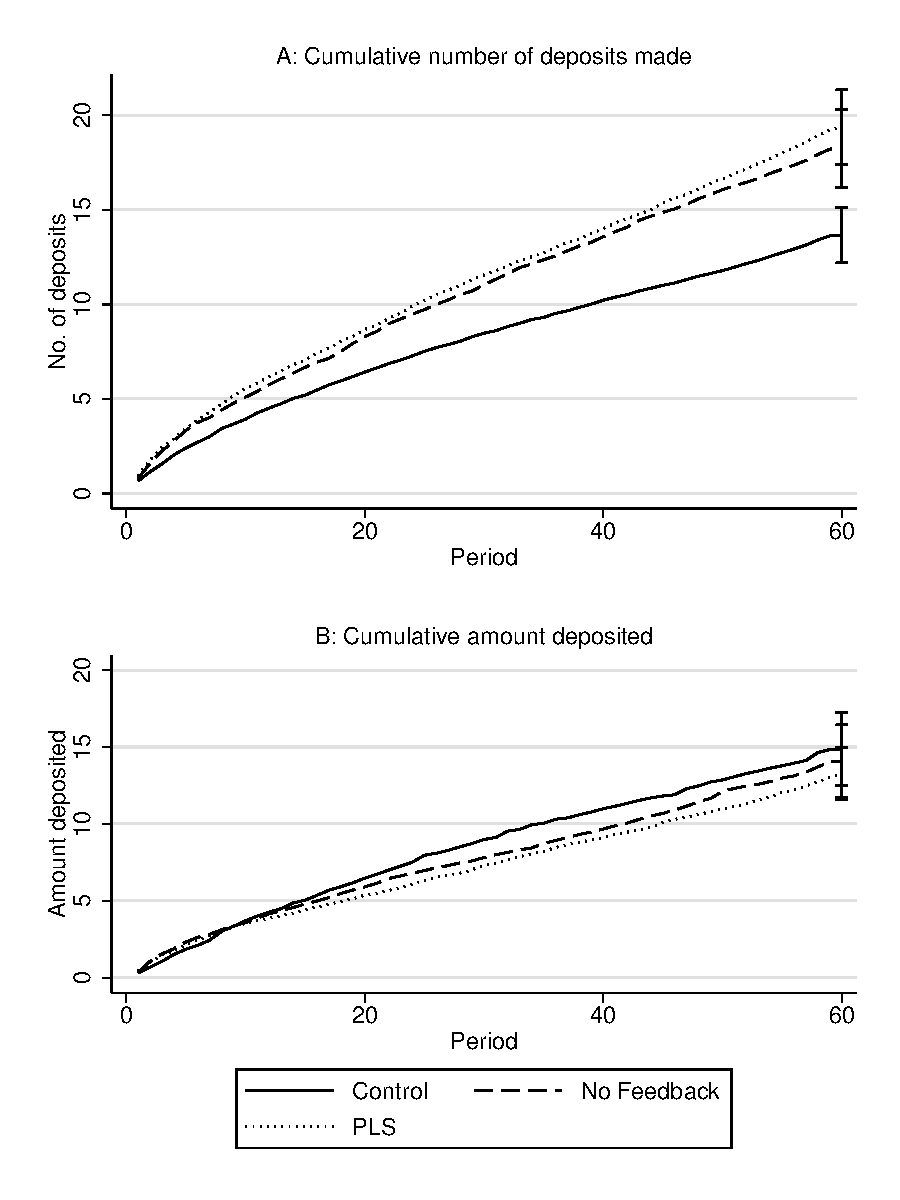
\includegraphics{../../figures/line-cumdeposits.pdf}
}

\end{frame}

\begin{frame} \frametitle{Treatment Effects -- Gross Deposits}
	
\maxsizebox*{0.90\linewidth}{0.90\paperheight}{
		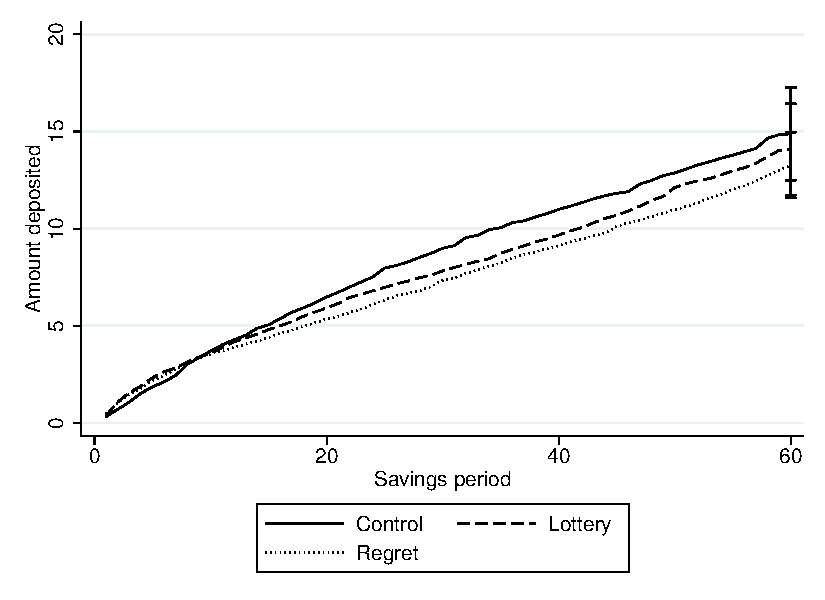
\includegraphics{../../figures/line-cumdepositamount.pdf}
}

\end{frame}

\begin{frame} \frametitle{Treatment Effects -- Mobile Savings}
	
	\begin{landscape} \begin{table}[htbp]\centering \def\sym#1{\ifmmode^{#1}\else\(^{#1}\)\fi} \label{tab:reg-mobile} \maxsizebox*{0.90\textwidth}{0.90\textheight}{ \begin{threeparttable} \begin{tabular}{l*{8}{c}} \toprule
          &\multicolumn{3}{c}{No controls}&\multicolumn{3}{c}{With controls}&\multicolumn{2}{c}{Sample}\\\cmidrule(lr){2-4}\cmidrule(lr){5-7}\cmidrule(lr){8-9}
          &\multicolumn{1}{c}{(1)}&\multicolumn{1}{c}{(2)}&\multicolumn{1}{c}{(3)}&\multicolumn{1}{c}{(4)}&\multicolumn{1}{c}{(5)}&\multicolumn{1}{c}{(6)}&\multicolumn{1}{c}{(7)}&\multicolumn{1}{c}{(8)}\\
          &\multicolumn{1}{c}{Lottery}&\multicolumn{1}{c}{Regret}&\multicolumn{1}{c}{\specialcell{Difference\\\(p\)-value}}&\multicolumn{1}{c}{Lottery}&\multicolumn{1}{c}{Regret}&\multicolumn{1}{c}{\specialcell{Difference\\\(p\)-value}}&\multicolumn{1}{c}{\specialcell{Control Mean\\(SD)}}&\multicolumn{1}{c}{N}\\
\midrule
Total no. of deposits&4.59$^{*}$&5.71$^{**}$&     0.69&4.20$^{*}$&5.55$^{**}$&     0.63&    13.66&      311\\
          &   (2.52)&   (2.45)&         &   (2.51)&   (2.44)&         &  (15.08)&         \\
          &   [0.13]&[0.06]$^{*}$&         &   [0.17]&[0.06]$^{*}$&         &         &         \\
\bottomrule \end{tabular} \begin{tablenotes}[flushleft] \footnotesize \item  \end{tablenotes} \end{threeparttable} } \end{table}
 \end{landscape}

\end{frame}

\begin{frame} \frametitle{Treatment Effects -- Mobile Savings}
	
	\begin{landscape} \begin{table}[htbp]\centering \def\sym#1{\ifmmode^{#1}\else\(^{#1}\)\fi} \label{tab:reg-mobile} \maxsizebox*{0.90\textwidth}{0.90\textheight}{ \begin{threeparttable} \begin{tabular}{l*{8}{c}} \toprule
          &\multicolumn{3}{c}{No controls}&\multicolumn{3}{c}{With controls}&\multicolumn{2}{c}{Sample}\\\cmidrule(lr){2-4}\cmidrule(lr){5-7}\cmidrule(lr){8-9}
          &\multicolumn{1}{c}{(1)}&\multicolumn{1}{c}{(2)}&\multicolumn{1}{c}{(3)}&\multicolumn{1}{c}{(4)}&\multicolumn{1}{c}{(5)}&\multicolumn{1}{c}{(6)}&\multicolumn{1}{c}{(7)}&\multicolumn{1}{c}{(8)}\\
          &\multicolumn{1}{c}{Lottery}&\multicolumn{1}{c}{Regret}&\multicolumn{1}{c}{\specialcell{Difference\\\(p\)-value}}&\multicolumn{1}{c}{Lottery}&\multicolumn{1}{c}{Regret}&\multicolumn{1}{c}{\specialcell{Difference\\\(p\)-value}}&\multicolumn{1}{c}{\specialcell{Control Mean\\(SD)}}&\multicolumn{1}{c}{N}\\
\midrule
Total no. of deposits&4.59$^{*}$&5.71$^{**}$&     0.69&4.20$^{*}$&5.55$^{**}$&     0.63&    13.66&      311\\
          &   (2.52)&   (2.45)&         &   (2.51)&   (2.44)&         &  (15.08)&         \\
          &   [0.13]&[0.06]$^{*}$&         &   [0.17]&[0.06]$^{*}$&         &         &         \\
No. of days saved&3.93$^{*}$&4.94$^{**}$&     0.66&3.49$^{*}$&4.76$^{**}$&     0.58&    11.78&      311\\
          &   (2.05)&   (2.08)&         &   (2.02)&   (2.09)&         &  (12.93)&         \\
          &   [0.13]&[0.04]$^{**}$&         &   [0.17]&[0.06]$^{*}$&         &         &         \\
\bottomrule \end{tabular} \begin{tablenotes}[flushleft] \footnotesize \item  \end{tablenotes} \end{threeparttable} } \end{table}
 \end{landscape}

\end{frame}

\begin{frame} \frametitle{Treatment Effects -- Mobile Savings}
	
	\begin{landscape} \begin{table}[htbp]\centering \def\sym#1{\ifmmode^{#1}\else\(^{#1}\)\fi} \label{tab:reg-mobile} \maxsizebox*{0.90\textwidth}{0.90\textheight}{ \begin{threeparttable} \begin{tabular}{l*{8}{c}} \toprule
          &\multicolumn{3}{c}{No controls}&\multicolumn{3}{c}{With controls}&\multicolumn{2}{c}{Sample}\\\cmidrule(lr){2-4}\cmidrule(lr){5-7}\cmidrule(lr){8-9}
          &\multicolumn{1}{c}{(1)}&\multicolumn{1}{c}{(2)}&\multicolumn{1}{c}{(3)}&\multicolumn{1}{c}{(4)}&\multicolumn{1}{c}{(5)}&\multicolumn{1}{c}{(6)}&\multicolumn{1}{c}{(7)}&\multicolumn{1}{c}{(8)}\\
          &\multicolumn{1}{c}{Lottery}&\multicolumn{1}{c}{Regret}&\multicolumn{1}{c}{\specialcell{Difference\\\(p\)-value}}&\multicolumn{1}{c}{Lottery}&\multicolumn{1}{c}{Regret}&\multicolumn{1}{c}{\specialcell{Difference\\\(p\)-value}}&\multicolumn{1}{c}{\specialcell{Control Mean\\(SD)}}&\multicolumn{1}{c}{N}\\
\midrule
Total no. of deposits&4.59$^{*}$&5.71$^{**}$&     0.69&4.20$^{*}$&5.55$^{**}$&     0.63&    13.66&      311\\
          &   (2.52)&   (2.45)&         &   (2.51)&   (2.44)&         &  (15.08)&         \\
          &   [0.13]&[0.06]$^{*}$&         &   [0.17]&[0.06]$^{*}$&         &         &         \\
No. of days saved&3.93$^{*}$&4.94$^{**}$&     0.66&3.49$^{*}$&4.76$^{**}$&     0.58&    11.78&      311\\
          &   (2.05)&   (2.08)&         &   (2.02)&   (2.09)&         &  (12.93)&         \\
          &   [0.13]&[0.04]$^{**}$&         &   [0.17]&[0.06]$^{*}$&         &         &         \\
Avg. no. of deposits&0.08$^{*}$&0.10$^{**}$&     0.69&0.07$^{*}$&0.09$^{**}$&     0.63&     0.23&      311\\
          &   (0.04)&   (0.04)&         &   (0.04)&   (0.04)&         &   (0.25)&         \\
          &   [0.13]&[0.06]$^{*}$&         &   [0.17]&[0.06]$^{*}$&         &         &         \\
\bottomrule \end{tabular} \begin{tablenotes}[flushleft] \footnotesize \item  \end{tablenotes} \end{threeparttable} } \end{table}
 \end{landscape}

\end{frame}

\begin{frame} \frametitle{Treatment Effects -- Mobile Savings}
	
	\begin{landscape} \begin{table}[h]\centering \def\sym#1{\ifmmode^{#1}\else\(^{#1}\)\fi} \label{tab:reg-mobile} \maxsizebox*{\textwidth}{\textheight}{ \begin{threeparttable} \begin{tabular}{l*{5}{c}} \toprule
          &\multicolumn{3}{c}{Effect estimates}&\multicolumn{2}{c}{Sample}\\\cmidrule(lr){2-4}\cmidrule(lr){5-6}
          &\multicolumn{1}{c}{(1)}&\multicolumn{1}{c}{(2)}&\multicolumn{1}{c}{(3)}&\multicolumn{1}{c}{(4)}&\multicolumn{1}{c}{(5)}\\
          &\multicolumn{1}{c}{No Feedback}&\multicolumn{1}{c}{PLS}&\multicolumn{1}{c}{\specialcell{PLS-\\No Feedback}}&\multicolumn{1}{c}{\specialcell{Control Mean\\(SD)}}&\multicolumn{1}{c}{Obs.}\\
\midrule
Total no. of deposits&4.59\sym{*}&5.71\sym{**}&     1.13&    13.66&      311\\
          &   (2.52)&   (2.45)&   (2.84)&  (15.08)&         \\
No. of days saved&3.93\sym{*}&4.94\sym{**}&     1.01&    11.78&      311\\
          &   (2.05)&   (2.08)&   (2.32)&  (12.93)&         \\
Total deposit amount&    -0.79&    -1.60&    -0.81&    14.87&      311\\
          &   (3.34)&   (2.91)&   (2.88)&  (24.48)&         \\
Total withdrawal amount&     0.53&1.63\sym{**}&     1.10&     1.07&      311\\
          &   (0.94)&   (0.74)&   (1.02)&   (4.53)&         \\
\bottomrule \end{tabular} \begin{tablenotes}[flushleft] \footnotesize \item  \end{tablenotes} \end{threeparttable} } \end{table}
 \end{landscape}

\end{frame}

% each row are results for each row variable as dependant variable
% column 1 is the coefficient on lottery etc.
% 40% more deposits over the project period than the matching incentive
% might expect an increase in no. of days in which they make non-zero deposits
% number of deposits per day increases as well
% column 3 tests whether the coefficients are the same, we cant reject the h but magnitudes suggest that it may contribute to the effect
% the second set of columns is the regression with controls
% robust to the inclusion of controls in the rhs
% se are in parentheses and fwer p-values are in the brackets to correct for multiple testing

\begin{frame} \frametitle{Treatment Effects -- Gambling}
	
	How do lottery-like incentives change outside gambling behavior?

\end{frame}

\begin{frame} \frametitle{Treatment Effects -- Gambling}

	\begin{landscape} \begin{table}[htbp]\centering \def\sym#1{\ifmmode^{#1}\else\(^{#1}\)\fi} \label{tab:reg-gamble} \maxsizebox*{0.90\textwidth}{0.90\textheight}{ \begin{threeparttable} \begin{tabular}{l*{8}{c}} \toprule
          &\multicolumn{3}{c}{No controls}&\multicolumn{3}{c}{With controls}&\multicolumn{2}{c}{Sample}\\\cmidrule(lr){2-4}\cmidrule(lr){5-7}\cmidrule(lr){8-9}
          &\multicolumn{1}{c}{(1)}&\multicolumn{1}{c}{(2)}&\multicolumn{1}{c}{(3)}&\multicolumn{1}{c}{(4)}&\multicolumn{1}{c}{(5)}&\multicolumn{1}{c}{(6)}&\multicolumn{1}{c}{(7)}&\multicolumn{1}{c}{(8)}\\
          &\multicolumn{1}{c}{Lottery}&\multicolumn{1}{c}{Regret}&\multicolumn{1}{c}{\specialcell{Difference\\\(p\)-value}}&\multicolumn{1}{c}{Lottery}&\multicolumn{1}{c}{Regret}&\multicolumn{1}{c}{\specialcell{Difference\\\(p\)-value}}&\multicolumn{1}{c}{\specialcell{Control Mean\\(SD)}}&\multicolumn{1}{c}{Obs.}\\
\midrule
Gamble more&     0.06&0.15$^{***}$&     0.16&     0.06&0.16$^{***}$&0.10$^{*}$&     0.12&      284\\
          &   (0.05)&   (0.06)&         &   (0.05)&   (0.05)&         &   (0.32)&         \\
          &   [0.80]&   [0.10]&         &   [0.90]&[0.00]$^{***}$&         &         &         \\
Gamble less&    -0.02&     0.04&     0.24&    -0.02&     0.03&     0.33&     0.16&      284\\
          &   (0.05)&   (0.06)&         &   (0.05)&   (0.06)&         &   (0.37)&         \\
          &   [0.90]&   [0.90]&         &   [0.90]&   [0.90]&         &         &         \\
More tempted to gamble&     0.09&     0.05&     0.56&     0.05&     0.03&     0.74&     0.47&      284\\
          &   (0.07)&   (0.07)&         &   (0.07)&   (0.07)&         &   (0.50)&         \\
          &   [0.70]&   [0.90]&         &   [0.90]&   [0.90]&         &         &         \\
Less tempted to gamble&    -0.01&     0.03&     0.27&    -0.00&     0.04&     0.30&     0.06&      284\\
          &   (0.03)&   (0.04)&         &   (0.03)&   (0.04)&         &   (0.25)&         \\
          &   [0.90]&   [0.80]&         &   [1.00]&   [0.70]&         &         &         \\
\bottomrule \end{tabular} \begin{tablenotes}[flushleft] \footnotesize \item  \end{tablenotes} \end{threeparttable} } \end{table}
 \end{landscape}

\end{frame}

\begin{frame} \frametitle{Discussion} \pause

	\begin{itemize}
	\item What is the appeal of lottery-like savings? \pause
		\begin{itemize}
		\item Lump-sum utility from gambling \pause
		\end{itemize}
	\item Are LLDAs useful? \pause
		\begin{itemize}
		\item More frequent deposits might be habit-forming \pause
		\item Could attract new savers to open accounts \pause
		\item Not revenue neutral if high transaction costs \pause
		\item Effect on outside gambling depends on program components (Cookson 2016) \pause
		\end{itemize}
	\end{itemize}

\end{frame}

% increased deposits but no increase in savings: are lottery incentives still useful?
% if habit forming, then it might be useful to more carefully track other savings and over a longer period of time
% one thing we didn't show is that we asked respondents at endline to self-select into one the the treatment groups, majority chose the lottery regardless of assignment
% cost on the financial institution perspective
% obviously, program components matter in how we design programs

\begin{frame} \frametitle{Conclusion} \pause
	
	\begin{itemize}
	\item What we find
		\begin{enumerate}
		\item More frequent deposits \pause
		\item No change in amount saved \pause
		\item Increase in self-reported gambling \pause
		\end{enumerate}
	\item To-do
		\begin{enumerate}
		\item Examine entire savings portfolio \pause
		\item Long term follow-up \pause
		\end{enumerate}
	\end{itemize}

\end{frame}

\begin{frame} \frametitle{Thank You}

	\begin{itemize}
	\item Research assistance
		\begin{itemize}
		\item Arun Varghese, Jonathan Page
		\end{itemize}
	\item Fieldwork
		\begin{itemize}	
		\item Busara Center For Behavioral Economics
		\end{itemize}
	\end{itemize}
\end{frame}

\appendix

\begin{frame} \frametitle{Appendix -- Attrition}
	
	\begin{table}[htbp]\centering \def\sym#1{\ifmmode^{#1}\else\(^{#1}\)\fi} \caption{Treatment group by participation at endline} \label{tab:tab-balance} \maxsizebox*{\paperwidth}{\paperheight}{ \begin{threeparttable} \begin{tabular}{l*{3}{c}} \toprule
                    &\multicolumn{3}{c}{Participation in endline}                     \\\cmidrule(lr){2-4}
                    &    Attrited         &   Completed         &       Total         \\
\midrule
Interest            &          11         &          94         &         105         \\
                    &                     &                     &                     \\
\addlinespace
Lottery             &           8         &          95         &         103         \\
                    &                     &                     &                     \\
\addlinespace
Regret              &           8         &          95         &         103         \\
                    &                     &                     &                     \\
\addlinespace
Total               &          27         &         284         &         311         \\
                    &                     &                     &                     \\
\bottomrule \end{tabular} \begin{tablenotes}[flushleft] \footnotesize \item \emph{Notes:} This table reports a cross-tabulation between treatment assignment and selection into the endline survey. \end{tablenotes} \end{threeparttable} } \end{table}


\end{frame}

\begin{frame} \frametitle{Appendix -- Attrition}
	
	\begin{table}[htbp]\centering \def\sym#1{\ifmmode^{#1}\else\(^{#1}\)\fi} \caption{Attrition by treatment group} \label{tab:reg-attr} \maxsizebox*{\paperwidth}{\paperheight}{ \begin{threeparttable} \begin{tabular}{l*{1}{c}} \toprule
                &\multicolumn{1}{c}{Unobserved at endline}\\
\midrule
Lottery         &    -0.03         \\
                &   (0.04)         \\
Regret          &    -0.03         \\
                &   (0.04)         \\
Constant        &     0.10\sym{***}\\
                &   (0.03)         \\
\midrule
Observations    &      311         \\
Adjusted \(R^{2}\)&   -0.004         \\
Difference p-value&     1.00         \\
Joint p-value   &     0.75         \\
\bottomrule \end{tabular} \begin{tablenotes}[flushleft] \footnotesize \item \emph{Notes:} This table reports a regression of selection on each of the treatment arms. Standard errors are in parentheses. * denotes significance at 10 pct., ** at 5 pct., and *** at 1 pct. level. \end{tablenotes} \end{threeparttable} } \end{table}

% File produced by akiba-estimate.do with /Users/Justin/Repos/akiba-lottery-pub/data/clean/akiba_wide.dta on 17:14:52 25 Mar 2017 by user Justin on Stata 13.1 with seed X53d8cd0fc43f462544a474abacbdd93d00044a8f

\end{frame}

\begin{frame} \frametitle{Appendix -- Baseline Balance}

		\begin{table}[h]\centering \def\sym#1{\ifmmode^{#1}\else\(^{#1}\)\fi} \caption{Baseline balance check by treatment group} \label{tab:sum-ysum1} \maxsizebox*{\textwidth}{\textheight}{ \begin{threeparttable} \begin{tabular}{l*{5}{c}} \toprule
          &\multicolumn{1}{c}{(1)}&\multicolumn{1}{c}{(2)}&\multicolumn{1}{c}{(3)}&\multicolumn{1}{c}{(4)}&\multicolumn{1}{c}{(5)}\\
          &\multicolumn{1}{c}{\specialcell{Lottery -\\Control}}&\multicolumn{1}{c}{\specialcell{Regret -\\Control}}&\multicolumn{1}{c}{\specialcell{Lottery -\\Regret}}&\multicolumn{1}{c}{\specialcell{Control mean\\(SD)}}&\multicolumn{1}{c}{Obs.}\\
\midrule
Female    &     0.07&     0.10&    -0.03&     0.52&      311\\
          &   (0.07)&   (0.07)&   (0.07)&   (0.50)&         \\
Age       &     0.78&     0.72&     0.05&    30.75&      303\\
          &   (1.39)&   (1.34)&   (1.36)&   (9.83)&         \\
Completed std. 8&    -0.02&    -0.02&    -0.00&     0.99&      311\\
          &   (0.02)&   (0.02)&   (0.02)&   (0.10)&         \\
Married/co-habitating&     0.10&     0.09&     0.01&     0.42&      307\\
          &   (0.07)&   (0.07)&   (0.07)&   (0.50)&         \\
No. of children&     0.23&     0.24&    -0.01&     1.75&      311\\
          &   (0.24)&   (0.25)&   (0.25)&   (1.70)&         \\
Coefficient of relative risk aversion&     0.08&    -0.03&     0.12&     1.16&      311\\
          &   (0.18)&   (0.17)&   (0.18)&   (1.27)&         \\
Locus of control&     0.48&    -0.83&     1.31&    69.81&      311\\
          &   (1.40)&   (1.46)&   (1.37)&  (10.78)&         \\
\bottomrule \end{tabular} \begin{tablenotes}[flushleft] \footnotesize \item \emph{Notes:} The first three columns report the difference of means across treatment groups with SEs in parentheses. Column 4 reports the mean of the control group with SD in parentheses. * denotes significance at 10 pct., ** at 5 pct., and *** at 1 pct. level. \end{tablenotes} \end{threeparttable} } \end{table}

% File produced by sum-treat.do with /Users/Justin/Repos/akiba-lottery-pub/data/clean/akiba_wide.dta on 22:18:49 15 Feb 2018 by user Justin on Stata 13.1 with seed X53d8cd0fc43f462544a474abacbdd93d00044a8f

\end{frame}

\begin{frame} \frametitle{Appendix -- Baseline Balance}

		\begin{table}[htbp]\centering \def\sym#1{\ifmmode^{#1}\else\(^{#1}\)\fi} \caption{Summary statistics by treatment group} \label{tab:sum-ysum2} \maxsizebox*{\textwidth}{\textheight}{ \begin{threeparttable} \begin{tabular}{l*{6}{c}} \toprule
          &\multicolumn{3}{c}{Mean (SD, N)}&\multicolumn{3}{c}{\specialcell{Difference\\\emph{p}-value}}\\\cmidrule(lr){2-4}\cmidrule(lr){5-7}
          &\multicolumn{1}{c}{Control}&\multicolumn{1}{c}{Lottery}&\multicolumn{1}{c}{Regret}&\multicolumn{1}{c}{\specialcell{Lottery -\\Control}}&\multicolumn{1}{c}{\specialcell{Regret -\\Control}}&\multicolumn{1}{c}{\specialcell{Lottery -\\Regret}}\\
\midrule
Monthly income&   112.05&   108.37&   111.46&     0.84&     0.97&     0.84\\
          &(137.13) 105&(117.43) 103&(104.85) 103&         &         &         \\
Receives regular income&     0.06&     0.11&     0.17&     0.36&0.08$^{*}$&     0.38\\
          &(0.24) 52&(0.31) 56&(0.38) 48&         &         &         \\
Employed  &     0.50&     0.54&     0.47&     0.49&     0.68&     0.27\\
          &(0.50) 105&(0.50) 103&(0.50) 103&         &         &         \\
Self-employed&     0.24&     0.21&     0.20&     0.61&     0.49&     0.87\\
          &(0.43) 78&(0.41) 72&(0.40) 81&         &         &         \\
No. of dependants&     3.18&     3.49&     3.27&     0.40&     0.79&     0.53\\
          &(2.58) 105&(2.60) 103&(2.32) 103&         &         &         \\
Subject is a dependant&     0.23&     0.28&     0.25&     0.38&     0.69&     0.64\\
          &(0.42) 105&(0.45) 103&(0.44) 103&         &         &         \\
\bottomrule \end{tabular} \begin{tablenotes}[flushleft] \footnotesize \item \emph{Notes:} The first three columns report means of each row variable for each treatment group. SD are in parentheses with sample size. The last three columns report the \emph{p}-value for a difference of means \emph{t}-test between each group. * denotes significance at 10 pct., ** at 5 pct., and *** at 1 pct. level. \end{tablenotes} \end{threeparttable} } \end{table}


\end{frame}

\begin{frame} \frametitle{Appendix -- Baseline Balance}

		\begin{table}[htbp]\centering \def\sym#1{\ifmmode^{#1}\else\(^{#1}\)\fi} \caption{Summary statistics by treatment group} \label{tab:sum-ysum3} \maxsizebox*{\textwidth}{\textheight}{ \begin{threeparttable} \begin{tabular}{l*{6}{c}} \toprule
          &\multicolumn{3}{c}{Mean (SD, N)}&\multicolumn{3}{c}{\specialcell{Difference\\\emph{p}-value}}\\\cmidrule(lr){2-4}\cmidrule(lr){5-7}
          &\multicolumn{1}{c}{Control}&\multicolumn{1}{c}{Lottery}&\multicolumn{1}{c}{Regret}&\multicolumn{1}{c}{\specialcell{Lottery -\\Control}}&\multicolumn{1}{c}{\specialcell{Regret -\\Control}}&\multicolumn{1}{c}{\specialcell{Lottery -\\Regret}}\\
\midrule
Currently saves&     0.56&     0.61&     0.47&     0.47&     0.17&0.04$^{**}$\\
          &(0.50) 105&(0.49) 103&(0.50) 103&         &         &         \\
Total savings last mo.&    58.82&    41.01&    51.79&     0.14&     0.58&     0.25\\
          &(106.26) 105&(59.72) 103&(72.56) 103&         &         &         \\
Currently saves with ROSCA&     0.58&     0.57&     0.66&     0.91&     0.24&     0.20\\
          &(0.50) 105&(0.50) 103&(0.48) 103&         &         &         \\
ROSCA savings last mo.&    13.83&    15.46&    15.92&     0.65&     0.52&     0.90\\
          &(23.24) 105&(28.42) 103&(23.41) 103&         &         &         \\
M-Pesa savings last mo.&     8.73&    17.24&     5.48&     0.35&     0.37&     0.18\\
          &(30.53) 105&(87.04) 103&(20.51) 103&         &         &         \\
\bottomrule \end{tabular} \begin{tablenotes}[flushleft] \footnotesize \item \emph{Notes:} The first three columns report means of each row variable for each treatment group. SD are in parentheses with sample size. The last three columns report the \emph{p}-value for a difference of means \emph{t}-test between each group. * denotes significance at 10 pct., ** at 5 pct., and *** at 1 pct. level. \end{tablenotes} \end{threeparttable} } \end{table}

% File produced by sum-treat.do with /Users/Justin/Repos/akiba-lottery-pub/data/clean/akiba_wide.dta on 14:45:02 12 Apr 2017 by user Justin on Stata 13.1 with seed X53d8cd0fc43f462544a474abacbdd93d00044a8f

\end{frame}

\begin{frame} \frametitle{Appendix -- Lottery Results}

	\begin{table}[htbp]\centering \def\sym#1{\ifmmode^{#1}\else\(^{#1}\)\fi} \caption{Expected and observed lottery results} \label{tab:tab-lottery} \maxsizebox*{\paperwidth}{\paperheight}{ \begin{threeparttable} \begin{tabular}{l*{3}{c}} \toprule
                    &        Freq.&         Pct. observed&      Pct. expected\\
\midrule
No match                   &        7065&       81.49&       62.43\\
One match                   &        1518&       17.51&       22.22\\
Two matches                   &          86&        0.99&       1.23\\
Complete match                   &           1&        0.01&      0.00\\
\bottomrule \end{tabular} \begin{tablenotes}[flushleft] \footnotesize \item \emph{Notes:} The first column tabulates the frequency of observed lottery ticket matches. The second and third columns report the observed and expected probabilities, respectively, of each type of lottery match. A lottery ticket was a random sequence of four numbers between 1 and 9, inclusive. Prizes were awarded according to how well a participant's lottery numbers matched the winning numbers. If the first or second numbers matched, a 10\% match of savings was awarded. If \emph{both} the first and second numbers matched, a 100\% match of savings was awarded. Finally if all numbers matched, a prize of 200 times the daily savings was awarded. \end{tablenotes} \end{threeparttable} } \end{table}


\end{frame}

\begin{frame} \frametitle{Appendix -- Estimation Strategy}

		$$ y_{i,E} = \beta_{0} + \beta_{1}\text{LOTTERY}_{i} + \beta_{2}\text{REGRET}_{i} + \delta y_{i,B} + \mathbf{X}'_i \omega + \varepsilon_{i} $$

		\begin{align*} y_{i,E} & \text{: Outcome at endline} \\
						\text{LOTTERY}_{i} & \text{: Lottery group} \\
						\text{REGRET}_{i} & \text{: Lottery with regret group} \\
						y_{i,B} & \text{: Outcome at baseline} \\
						\mathbf{X}_i & \text{: Controls} \\
		\end{align*}

\end{frame}

\begin{frame} \frametitle{Appendix -- Mobile savings by period}

	\begin{landscape} \begin{table}[h]\centering \def\sym#1{\ifmmode^{#1}\else\(^{#1}\)\fi} \label{tab:reg-panel} \maxsizebox*{\textwidth}{\textheight}{ \begin{threeparttable} \begin{tabular}{l*{5}{c}} \toprule
          &\multicolumn{3}{c}{Effect estimates}&\multicolumn{2}{c}{Sample}\\\cmidrule(lr){2-4}\cmidrule(lr){5-6}
          &\multicolumn{1}{c}{(1)}&\multicolumn{1}{c}{(2)}&\multicolumn{1}{c}{(3)}&\multicolumn{1}{c}{(4)}&\multicolumn{1}{c}{(5)}\\
          &\multicolumn{1}{c}{No Feedback}&\multicolumn{1}{c}{PLS}&\multicolumn{1}{c}{\specialcell{PLS-\\No Feedback}}&\multicolumn{1}{c}{\specialcell{Control Mean\\(SD)}}&\multicolumn{1}{c}{Obs.}\\
\midrule
No. of deposits made&0.08\sym{*}&0.09\sym{**}&     0.02&     0.23&    18636\\
          &   (0.04)&   (0.04)&   (0.05)&   (0.51)&         \\
Made a deposit&0.07\sym{*}&0.08\sym{**}&     0.02&     0.20&    18660\\
          &   (0.03)&   (0.03)&   (0.04)&   (0.40)&         \\
Amount deposited&    -0.01&    -0.03&    -0.01&     0.25&    18636\\
          &   (0.06)&   (0.05)&   (0.05)&   (1.03)&         \\
Amount withdrew&     0.01&0.03\sym{**}&     0.02&     0.02&    18636\\
          &   (0.02)&   (0.01)&   (0.02)&   (0.60)&         \\
\bottomrule \end{tabular} \begin{tablenotes}[flushleft] \footnotesize \item  \end{tablenotes} \end{threeparttable} } \end{table}
 \end{landscape}

\end{frame}

\begin{frame} \frametitle{Appendix -- Other Savings}

	\begin{landscape} \begin{table}[htbp]\centering \def\sym#1{\ifmmode^{#1}\else\(^{#1}\)\fi} \label{tab:reg-save} \maxsizebox*{0.90\textwidth}{0.90\textheight}{ \begin{threeparttable} \begin{tabular}{l*{8}{c}} \toprule
          &\multicolumn{3}{c}{No controls}&\multicolumn{3}{c}{With controls}&\multicolumn{2}{c}{Sample}\\\cmidrule(lr){2-4}\cmidrule(lr){5-7}\cmidrule(lr){8-9}
          &\multicolumn{1}{c}{(1)}&\multicolumn{1}{c}{(2)}&\multicolumn{1}{c}{(3)}&\multicolumn{1}{c}{(4)}&\multicolumn{1}{c}{(5)}&\multicolumn{1}{c}{(6)}&\multicolumn{1}{c}{(7)}&\multicolumn{1}{c}{(8)}\\
          &\multicolumn{1}{c}{Lottery}&\multicolumn{1}{c}{Regret}&\multicolumn{1}{c}{\specialcell{Difference\\\(p\)-value}}&\multicolumn{1}{c}{Lottery}&\multicolumn{1}{c}{Regret}&\multicolumn{1}{c}{\specialcell{Difference\\\(p\)-value}}&\multicolumn{1}{c}{\specialcell{Control Mean\\(SD)}}&\multicolumn{1}{c}{Obs.}\\
\midrule
Total savings last mo.&    18.45&   -17.87&     0.13&    16.75&   -12.44&     0.19&    80.31&      284\\
          &  (25.16)&  (14.64)&         &  (23.25)&  (14.86)&         & (112.74)&         \\
          &[0.00]$^{***}$&   [1.00]&         &   [1.00]&[0.00]$^{***}$&         &         &         \\
M-Pesa savings last mo.&    -5.42&    -6.71&     0.81&    -5.47&    -6.19&     0.89&    20.42&      284\\
          &   (6.34)&   (5.49)&         &   (6.06)&   (5.38)&         &  (44.67)&         \\
          &[0.00]$^{***}$&   [1.00]&         &   [1.00]&[0.00]$^{***}$&         &         &         \\
ROSCA savings last mo.&     1.48&     7.37&     0.42&     2.84&     7.85&     0.46&    22.24&      283\\
          &   (6.76)&   (6.79)&         &   (6.26)&   (6.35)&         &  (42.18)&         \\
          &   [1.00]&   [1.00]&         &   [1.00]&[0.00]$^{***}$&         &         &         \\
Currently saves with ROSCA&    -0.02&0.14$^{**}$&0.02$^{**}$&    -0.01&0.14$^{**}$&0.03$^{**}$&     0.54&      284\\
          &   (0.07)&   (0.07)&         &   (0.07)&   (0.06)&         &   (0.50)&         \\
          &   [1.00]&   [1.00]&         &   [1.00]&[0.00]$^{***}$&         &         &         \\
\bottomrule \end{tabular} \begin{tablenotes}[flushleft] \footnotesize \item  \end{tablenotes} \end{threeparttable} } \end{table}
 \end{landscape}

\end{frame}

\begin{frame} \frametitle{Appendix -- Heterogeneity}

	\begin{table}[htbp]\centering \def\sym#1{\ifmmode^{#1}\else\(^{#1}\)\fi} \caption{Heterogeneous effects - Primary outcomes by female} \label{tab:het-demo_female_0} \maxsizebox*{\paperwidth}{\paperheight}{ \begin{threeparttable} \begin{tabular}{l*{4}{c}} \toprule
                &\multicolumn{1}{c}{(1)}&\multicolumn{1}{c}{(2)}&\multicolumn{1}{c}{(3)}&\multicolumn{1}{c}{(4)}\\
                &\multicolumn{1}{c}{Total no. of deposits}&\multicolumn{1}{c}{Daily avg. no. of deposits}&\multicolumn{1}{c}{No. of days saved}&\multicolumn{1}{c}{Gamble more}\\
\midrule
Lottery         &     4.62         &     0.08         &     4.21         &     0.16\sym{*}  \\
                &   (3.71)         &   (0.06)         &   (3.14)         &   (0.08)         \\
Lottery $\times$ \\ Female&     0.07         &     0.00         &    -0.41         &    -0.17         \\
                &   (5.06)         &   (0.08)         &   (4.16)         &   (0.11)         \\
Regret          &     0.33         &     0.01         &     0.67         &     0.19\sym{**} \\
                &   (3.57)         &   (0.06)         &   (3.07)         &   (0.09)         \\
Regret $\times$ \\ Female&     8.84\sym{*}  &     0.15\sym{*}  &     6.96\sym{*}  &    -0.07         \\
                &   (4.84)         &   (0.08)         &   (4.13)         &   (0.12)         \\
Female          &    -1.15         &    -0.02         &    -0.61         &     0.05         \\
                &   (2.98)         &   (0.05)         &   (2.55)         &   (0.07)         \\
Constant        &    14.26\sym{***}&     0.24\sym{***}&    12.10\sym{***}&     0.09\sym{**} \\
                &   (2.26)         &   (0.04)         &   (1.94)         &   (0.04)         \\
\midrule
Adjusted \(R^{2}\)&    0.015         &    0.015         &    0.016         &    0.016         \\
Control mean    &    13.66         &     0.23         &    11.78         &     0.12         \\
Lottery \emph{p}-value&     0.17         &     0.17         &     0.17         &     0.85         \\
Regret \emph{p}-value&     0.01         &     0.01         &     0.01         &     0.13         \\
Observations    &      311         &      311         &      311         &      284         \\
\bottomrule \end{tabular} \begin{tablenotes}[flushleft] \footnotesize \item \emph{Notes:} This table reports OLS estimates of the treatment effect and its interaction with baseline. Standard errors are in parentheses. * denotes significance at 10 pct., ** at 5 pct., and *** at 1 pct. level. We also report the \(p\)-values for joint tests on the direct treatment effect conditional on the baseline covariate $= 1$. \end{tablenotes} \end{threeparttable} } \end{table}

% File produced by akiba_estimate.do with /Users/Justin/Repos/akiba-lottery-pub/data/clean/akiba_wide.dta on 17:15:12 25 Mar 2017 by user Justin on Stata 13.1 with seed Xab009a28c79e3115499f664c1f29957300040c93

\end{frame}

\end{document} 